\documentclass{article}

\usepackage{graphicx}
\usepackage{tikz}
\usepackage{tikzsymbols}
\usetikzlibrary{calc,patterns,shapes.geometric}
\pagestyle{empty}
\usepackage[margin=0pt]{geometry}
\geometry{papersize={14in,12in}}

\def\centerarc[#1](#2)(#3:#4:#5){\draw[#1] ($(#2)+({#5*cos(#3)},{#5*sin(#3)})$) arc (#3:#4:#5);}

\begin{document}
	\begin{figure}
		\centering
		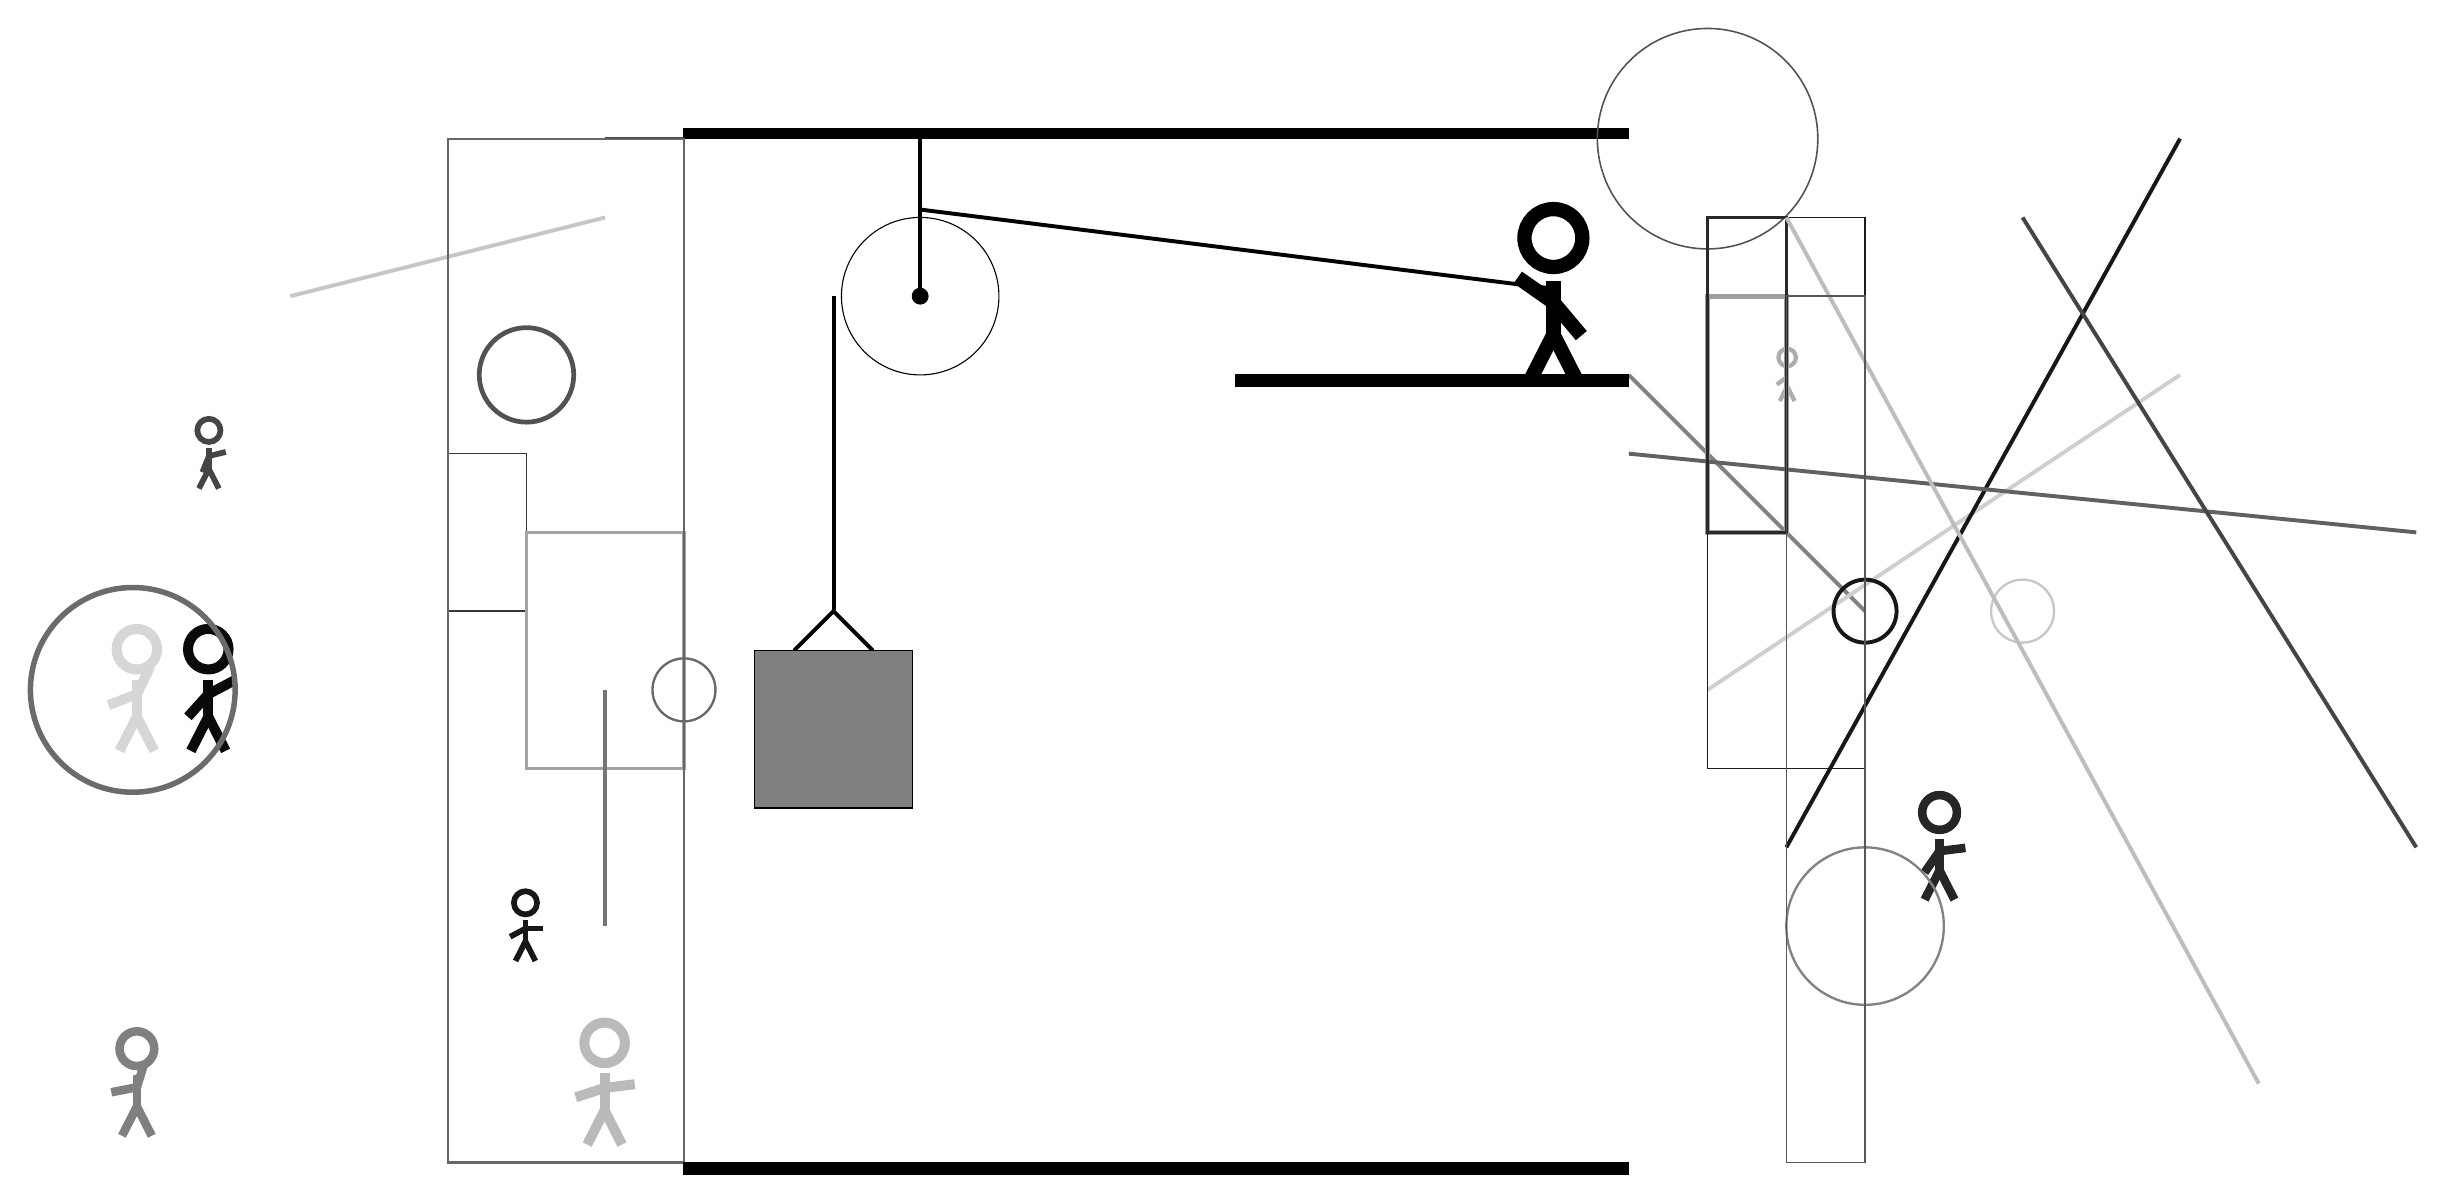
\begin{tikzpicture}
			%%%%% START %%%%%
			
			\draw[fill=black] (-2, 10) rectangle (10, 10.125);
			
			\draw[line width=0.2mm, color=black!79] (-4, 6) rectangle (-5, 4);
			
			\draw[line width=0.4mm, color=black!36] (-4, 2) rectangle (-2, 5);
			\draw[line width=0.5mm, color=black!50](10, 7) -- (13, 4);
			\draw[line width=0.5mm, color=black!19](11, 3) -- (17, 7);
			\draw [line width=0.2mm, color=black!68](11, 10) circle (1.4);
			
			\node[line width=0.4mm, color=black!50] at (-9, -2) {\Strichmaxerl[6][11][73]};
			\draw[line width=0.6mm, color=black!38] (12, 5) rectangle (11, 8);
			\draw [line width=0.5mm, color=black!91](13, 4) circle (0.4);
			\draw [line width=0.3mm, color=black!22](15, 4) circle (0.4);
			\draw[line width=0.2mm, color=black!89] (11, 9) rectangle (13, 2);
			
			\draw[line width=0.5mm, color=black!91](12, 1) -- (17, 10);
			\draw[line width=0.4mm, color=black!73] (-3, 10) rectangle (-2, 10);
			\draw[line width=0.5mm, color=black!62](10, 6) -- (20, 5);
			
			\node[line width=0.5mm, color=black!91] at (-4, 0) {\Strichmaxerl[4][28][0]};
			\draw[line width=0.5mm, color=black!54](-3, 3) -- (-3, 0);
			\node[line width=0.7mm, color=black!27] at (-3, -2) {\Strichmaxerl[7][18][7]};
			\node[line width=0.5mm, color=black!96] at (-8, 3) {\Strichmaxerl[7][48][28]};
			\node[line width=0.6mm, color=black!32] at (12, 7) {\Strichmaxerl[3][37][90]};
			\draw[line width=0.5mm, color=black!22](-7, 8) -- (-3, 9);
			\node[line width=0.3mm, color=black!73] at (-8, 6) {\Strichmaxerl[4][68][14]};
			\node[line width=0.6mm, color=black!85] at (14, 1) {\Strichmaxerl[6][55][7]};
			
			\draw[line width=0.4mm, color=black!84] (11, 5) rectangle (12, 9);
			
			\draw[line width=0.3mm, color=black!60] (-2, 10) rectangle (-5, -3);
			\draw[line width=0.5mm, color=black!26](12, 9) -- (18, -2);
			\node[line width=0.5mm, color=black!16] at (-9, 3) {\Strichmaxerl[7][21][64]};
			
			\draw [line width=0.3mm, color=black!49](13, 0) circle (1.0);
			
			\draw [line width=0.6mm, color=black!68](-4, 7) circle (0.6);
			\draw[line width=0.2mm, color=black!66] (12, 8) rectangle (13, -3);
			\draw[line width=0.5mm, color=black!73](15, 9) -- (20, 1);
			\draw [line width=0.3mm, color=black!59](-2, 3) circle (0.4);
			\draw [line width=0.7mm, color=black!58](-9, 3) circle (1.3);
			
			
			\draw (1, 8) circle (1);
			\draw[fill=black] (1, 8) circle (0.1);
			\draw[line width=0.5mm] (1, 10) -- (1, 8);
			
			\draw[line width=0.5mm](-0.6, 3.5) --  (-0.1, 4.0) -- (0.4, 3.5);
			\draw[fill=black!50] (-1.1, 3.5) rectangle (0.9, 1.5);
			
			\draw[line width=0.5mm](-0.1, 8) -- (-0.1, 4.0);
			\centerarc[line width=0.5mm](1, 8)(90:180:1.1)
			\draw[line width=0.5mm](1, 9.1) -- (9, 8.1);
			
			\node at (9, 8) {\Strichmaxerl[10][-35][-50]};
			\draw[fill=black] (5, 7) rectangle (10, 6.85);
			
			\draw[fill=black] (-2, -3) rectangle (10, -3.15);
			
			%%%%% END %%%%%
		\end{tikzpicture}
	\end{figure}	
\end{document}